%%%%%%%%%%%%%%%%%%%%%%%%%%%%%%%%%%%%%%%%%%%%%%%%%%%%%%%%%%%%%%%%%%%%%%%%
% Requires the installation of Microsoft fonts (Arial).
% Install on Linux with "sudo apt-get install ttf-mscorefonts-installer"
%%%%%%%%%%%%%%%%%%%%%%%%%%%%%%%%%%%%%%%%%%%%%%%%%%%%%%%%%%%%%%%%%%%%%%%%

\documentclass[11pt,a4paper]{article}

%%%%%%%%%%%%%%%%%%%%  packages and definitions %%%%%%%%%%%%%%%%%%%%%%%%%

\usepackage[margin=2cm]{geometry}

\usepackage{url}
\usepackage[hidelinks]{hyperref}
%\usepackage{cite}
\usepackage{xcolor}
\usepackage{tabularx}
\usepackage{booktabs} %for toprule, midrule of tab
\usepackage{siunitx}
\usepackage{setspace}
\setstretch{1.0} 
\usepackage{titlesec}
\usepackage{enumitem}
\setlist[itemize]{itemsep=4pt,parsep=2pt,topsep=2pt,leftmargin=0.5cm,labelsep=4pt}

\usepackage{amsmath,amssymb}

% setting Arial font
\usepackage{fontspec}
\usepackage{fontspec-luatex}
\setmainfont{Arial} 
% for Gantt charts
\usepackage{pgfgantt}
\usepackage{float}
\usepackage{cleveref}
\usepackage{csquotes}

\usepackage{graphicx}
\usepackage[font=footnotesize]{caption} 

% colors
\definecolor{barblue}{RGB}{153,204,254}
\definecolor{groupblue}{RGB}{51,102,254}
\definecolor{linkred}{RGB}{165,0,33}
\definecolor{linkgreen}{RGB}{20,182,117}
\definecolor{linkorange}{RGB}{205,134,41}
\definecolor{green}{RGB}{0, 128, 0}
\definecolor{red}{RGB}{255, 0, 0}
\definecolor{lightblue}{RGB}{173, 216, 230}
\definecolor{mydarkblue}{RGB}{0, 0, 139}
\definecolor{mydarkgreen}{RGB}{0, 100, 0}
\definecolor{mylightgreen}{RGB}{56, 93, 75}
\setganttlinklabel{s-s}{START-TO-START}
\setganttlinklabel{f-s}{FINISH-TO-START}
\setganttlinklabel{f-f}{FINISH-TO-FINISH}
\sffamily

\usepackage{array}
\newcolumntype{P}[1]{>{\raggedright\arraybackslash}p{#1}}
\usepackage{multirow}
\usepackage{pifont}
\usepackage{wasysym}
\usepackage{pstricks}
\usepackage{wasysym}

\usepackage[backend=bibtex, style=ieee, maxbibnames=99]{biblatex}
\addbibresource{refs/refs.bib}
\DeclareBibliographyCategory{dontbib}
\addtocategory{dontbib}{TPO, TPO2, TPO3, TPO4, TPOIRIM, LaserHumanoids, LaserJournal, Muratore2023, Bertoni2023, ROSEE, RoseePaper, RoseePaperLiana}
\preto\fullcite{\AtNextCite{\defcounter{maxnames}{99}}}

\author{Davide Torielli}
\title{Bioengineering and Robotics PhD annual report template}

\titleformat{\section}
{\bfseries\normalsize} % Formatting for the title (bold and large)
{\thesection.}     % Section number
{0.5em}        
     % Space between section number and title
{}                % Code before the title

\titleformat{\subsection}
{\normalsize} % Formatting for the title (bold and large)
{\thesubsection}     % Section number
{1em}        
% Space between section number and title
{}         

\begin{document}
\begin{figure}[t]
	\centering
	\includegraphics[width=0.99\textwidth]{logos/top_logos.pdf}
\end{figure}
\hphantom{h}\vspace{1.3cm}


\begin{center}
	
\LARGE{\textbf{PhD Program in Bioengineering and Robotics}\vspace{0.4cm}\\
Curriculum: Advanced and Humanoid Robotics}

\end{center}

\begin{flushleft}
\vspace{1.5cm}
\large{\textbf{Student: }}\large{{Torielli, Davide}}\vspace{0.2cm}\\
\large{\textbf{Cycle: }}\large{XXXVI}\vspace{0.2cm}\\
\large{\textbf{Tutors: }}\large{{Tsagarakis, Nikos and Muratore, Luca}}\vspace{0.2cm}\\
\large{\textbf{Year: }}\large{3$^{rd}$}\vspace{0.2cm}\\
\large{\textbf{Contacts: }}\large{{toridebraus@gmail.com}\qquad{davide.torielli@iit.it}}
\end{flushleft}
\clearpage
\begin{center}
	\textbf{\normalsize{Intuitive human-robot interfaces for the control of complex robots}}
\end{center}

\section{Objectives}
%  [max 1 page]
%%Motivate your research and define the general goal of the research project (i.e., which is the addressed S/T question?
%Detail the specific objectives of the current year, and summarize the planned activities of the other two/one years. 

Nowadays, the recent advancements in the development of robotic systems have augmented the robot capabilities, making it possible to face complex tasks. Indeed, in always more challenging scenarios, like industry and construction sites, robots can help the workers, relieving them from the most exhausting and dangerous part of their job, for example the manipulation of heavy loads in unstructured environments. 
The growing complexity of robots and the effective exploitation of their enhanced capabilities can be tackled by the development of novel intuitive human-robot interfaces. 

The objective of this research is indeed to explore and develop new human-robot interfaces that are intuitive and easy-to-use, minimizing the operator cognitive and physical workload while controlling a high-redundant robotic system. At the same time, the interfaces must deliver a certain level of robot autonomy, relieving the operator to take care of every minimal aspect of the task. 

Considering these key challenges, this research project explored new intuitive teleoperation paradigms.
One result is the development of the TelePhysicalOperation concept, an innovative teleoperation interface that combines the intuitiveness of a physical human-robot interaction maintaining the safety of controlling the robot from a distance.
The interface has been enriched with robot autonomy features to reduce the operator burden and to improve the performance of the task, in a shared-control fashion. For example, a mobile manipulator can generate arm and mobile base commands from a single input of the operator, relieving her/him to switch between arm and mobile base control. Thanks to another autonomy feature, the robot can bimanually keep the grasp on a transported load while the operator commands only the object velocities, without worrying about the grasping forces necessary to make the object to not fall. 

In general, it is not always straightforward for the operator to be aware about the status of the robot and of the task by visual information only, delivered by a monitor or by directly looking at the robot. For this reason, this research explored the importance of tactile feedback during the remote teleoperation. The TelePhysicalOperation interface has been improved by adding a feedback channel realized with the development of a customized sensorimotor interface. The integrated devices deliver indentation and vibrotactile feedback to the user's in response to inputs given to the robot and interactions with the robot's environment. This enhancement in the operator's experience has been validated involving novice TelePhysicalOperation users.

Another aspect of this work explored a teleoperation interface which relies on visual servoing guidance through a laser device. With the architecture developed, the operator, by pointing a laser emitter in the environment, is able to command target locations to even highly articulated robots effortlessly and efficiently for loco-manipulation tasks. The same interface has also been proved to be adaptable to a different scenario, an assistive one, where users with arm impairments can control a manipulator with the laser emitter worn on the head.    

In conclusion, this research has explored new kinds of interfaces to face the challenge of commanding complex robots but without overwhelming the operator with complicated user interfaces.
\newpage
\section{State of art and proposed innovation} 
% [max 1 page, max 20 refs]
%Properly frame the research in the literature. Which is the gap you plan to bridge? Which are the open issues you aim to address? 
%(If the objectives of the project do not change during the 3-years, this section could be filled only the first year and modified only by adding new relevant works published). 

Robotic teleoperation is one of the oldest fields in robotics~\cite{Goertz1952},⁠ but yet an active and evolving research topic. 
The increasing robot capabilities have expanded the possible application of teleoperation in very different areas such as in disaster response~\cite{Liu2013}⁠⁠, construction industry~\cite{Carra2018}, assistive scenarios~\cite{Petrich2022}, for permitting the remote command and execution of complex loco-manipulation tasks.
At the same time, the improved capabilities of recent mobile/legged manipulation platforms have increased the complexity of remotely commanding them, hence augmenting the burden of the operator in executing remote tasks. This has motivated works, which target to develop more intuitive and smarter interaction and commanding interfaces for the teleoperation the remotely operated robot.

Flexible interfaces that attempt to track multiple operator inputs have been explored, based on Inertial Measurement Unit (IMU) devices to direct teleoperate humanoids robots~\cite{Darvish23}. In these cases, the complexity of the slave robot is handled by sending multiple inputs provided by a sensorized full body interface. The work in~\cite{Wu2019}⁠ exploited a full body IMU-based suit combined with a human center of pressure model and a tele-impedance interface to control the locomotion and manipulation actions. Tele-impedance control enriches the command sent to the remote robot by combing the master estimated position and the stiffness references obtained through an Electromyography (EMG) interface~\cite{Ajoudani2012}⁠. Another class of approach for the teleoperation is the exploitation of exoskeletons with dissimilar kinematics respect to the robot to control~\cite{Rebelo2012}⁠. This introduces challenges in how to map the master and slave kinematics at best, and how to design the cumbersome exoskeleton interface to be more comfortable as possible when worn by the operator. Despite all the provided solutions for the teleoperation of complex loco-manipulation platforms, one of the most intuitive ways to guide the robot is by physically interacting with its body to drive it along the desired motion to teach or guide during collaborative tasks. Indeed, physical Human Robot Interaction (pHRI) can assist the operator in accomplishing collaborative tasks in collaboration with the robot~\cite{Cherubini2016, Kruger2009}⁠. 

To augment the robot autonomy, providing smarter teleoperation interface which permits to relieve the operator from commanding each aspect of the tasks, more intelligent human-robot teleoperation interfaces have been explored, providing various levels of shared control or shared autonomy~\cite{Selvaggio2021}. An idea is to give full autonomy to the robotic system to handle the \enquote{low-level} operations, while the human operator provides the \enquote{high-level} commands. This concept is supported by the fact that, for example, humans are better than machines in processing visual information, but they are prone to errors due to fatigue when a precise end-effector trajectory is needed~\cite{Yang2018}⁠. In some relevant works is shown that the teleoperated robot autonomously points the gripper in a specific direction~\cite{Abi2016}, overrides the commands of the human operator to avoid unsafe regions [17] and obstacles~\cite{Masone2018}, and maintains the dual-arm grasp on a transported object~\cite{Shahbazi2017, Laghi2018}, [C.3], [C.5].

In parallel, several works have coupled the remote robot control with a sensory feedback channel that supplements the visual domain, encompassing an array of stimuli like haptic cues to leverage the human sense of touch~\cite{Dargahi2004, Pacchierotti2015}. Wearable interfaces, in particular, allow to deliver a variety of cutaneous cues (e.g., skin stretch, vibration, temperature) to different body parts, resulting in unobtrusive and flexible devices capable of transmitting different kinds of information to the user~\cite{pacchierotti2017wearable}. 
%

Despite all the advancements in these technologies, it is still a challenge to develop a teleoperation interface that allows the control of complex robots while maintaining a simple structure, not overwhelming the operator with difficult-to-learn and cumbersome human robot interfaces. This is the key aspect of the research, which has explored new kind of intuitive teleoperation paradigms and validate them with complex mobile manipulators.
\section{Methodology and workplan}
% [max 1.5 page]

%Provide: 
%\begin{itemize}
%	\item[-] Overview of the proposed approach you plan to follow (including methods and techniques)
%	\item[-] List of tasks organized in tables (see below). (For each task, brief summary of the progress of the research accomplishments (the details about the results achieved will be provided in Sect. 4).
%	
%	Additionally, a Gantt chart is required (see below for an example).
%\begin{figure}[h]
%	\begin{center}
%		\begin{ganttchart}[
%			canvas/.append style={fill=none, draw=black!5, line width=.75pt},
%			hgrid style/.style={draw=black!40, line width=1.0pt},
%			vgrid={*1{draw=black!40, line width=1.0pt}},
%			today=11,
%			today rule/.style={
%				draw=black,
%				dash pattern=on 3.5pt off 4.5pt,
%				line width=1.8pt
%			},
%			y unit chart=1cm,
%			today label font=\footnotesize\bfseries,
%			title/.style={text=black, draw=black, fill=gray!30, font=\Large\bfseries, align=center},
%			title label font=\bfseries\footnotesize,
%			title label node/.append style={below=-7pt},
%			title left shift=0.0,
%			title top shift=0.2,
%			include title in canvas=false,
%			bar label font=\mdseries\small\color{black!90},
%			bar/.append style={draw=none, fill=blue!40},
%			bar incomplete/.append style={fill=lightblue!80},
%			bar height=0.2,
%			bar label node/.append style={left=0.2cm, fill=black!10},
%			bar progress label font=\bfseries\small,
%			bar progress label font=\mdseries\footnotesize\color{black!80},
%			%	progress label text={\si{\percent}},
%			group incomplete/.append style={fill=lightblue},
%			group/.append style={
%				fill=mydarkgreen!60, % Change this color for completed group bars
%			},
%			group left shift=0,
%			group right shift=0,
%			group label font=\mdseries\bfseries\small\color{black!90},
%			group height=.3,
%			group peaks tip position=0,
%			group label node/.append style={left=0.4cm, fill=black!20},
%			group progress label font=\mdseries\footnotesize\color{black!80},
%			]{1}{12}
%			\gantttitle[
%			title label node/.append style={below left=-7pt and -7pt}
%			]{Months:\quad1}{1}
%			\gantttitlelist{2,...,12}{1} \\
%			[grid]
%			\ganttgroup[progress=61]{Macro-task 1}{1}{10} \\
%			[grid]
%			\ganttbar[
%			progress=75,
%			name=subtask1
%			]{\textbf{Subtask 1.1}}{1}{8} \\
%			[grid]
%			\ganttbar[
%			progress=47,
%			name=subtask1
%			]{\textbf{Subtask 1.2}}{4}{10}
%		\end{ganttchart}
%	\end{center}
%	\caption{Example Gantt chart for your tasks.}
%\end{figure}
%
%\end{itemize}

To advance the state of the art in telerobotics, this research addresses key challenges such as enabling effortless control of complex robots, developing intuitive interfaces which includes robot autonomy features.
In the first period, the TelePhysicalOperation interface has been developed. Later, the interface has been enhanced with some robot autonomy features to \enquote{share the control} between the operator and the robot itself: for example, while the operator commands only the velocity of the end-effector, the robot generates arm commands and mobile base commands according to the arm manipulability level, letting the end-effector to reach the goal even if it is out of the reaching of the arm.
The interface has been further enriched by incorporating a haptic feedback channel, allowing users to perceive information beyond the visual domain. Naive users who evaluated the haptic-enabled TelePhysicalOperation positively endorsed the inclusion of haptic cues.

Concurrently, an alternative teleoperation interface has been developed, utilizing visual servoing guidance with a laser device. The resulting user interface is very easy-to-use and intuitive, requiring more robot autonomy which has been addressed with an architecture based on Behaviour Trees~\cite{Iovino2022}.
Other than with complex robots, the interface has been evaluated with a simpler fixed manipulator, but showing the potentiality of this interface as an assistive device for impaired arm users.
	
\begin{table}[H]
	\begin{center}
		\renewcommand{\arraystretch}{1.3} % Adjust the vertical spacing
		\setlength{\tabcolsep}{8pt} % Adjust the horizontal spacing
		\begin{tabular}{|P{15cm}|}
			\hline
			\textbf{Task name} Development of TelePhysicalOperation (TPO) \\ \hline
			\textbf{Scheduling}: Months 1-11 \\ \hline
			\textbf{Performed actions}: Studied the state of art regarding teleoperation, human-robot interaction, and master-slave hardware interfaces. 
			Developed Software Architecture for both control part and input interface 
			Evaluation experiments on real robot\\
			\hline
			\textbf{Achieved results}: A Control Interface to teleoperate complex robot has been developed. Test on real platform (CENTAURO) has been validated, resulting in a publication. Presentation at the ICRA22 conference \\
			\hline
			\textbf{Status}: Completed\\
			\hline
			\textbf{Publications relative to the task}: [J.1]\\
			\hline
			\textbf{Revised planning}\\
			\hline
		\end{tabular}
	\end{center}
\end{table}

\begin{table}[H]
	\begin{center}
		\renewcommand{\arraystretch}{1.3} % Adjust the vertical spacing
		\setlength{\tabcolsep}{8pt} % Adjust the horizontal spacing
		\begin{tabular}{|P{15cm}|}
			\hline
			\textbf{Task name} TPO: Shared Locomanipulation \\ \hline
			\textbf{Scheduling}: Months 11-21 \\ \hline
			\textbf{Performed actions}: Explored and developed autonomy modules and implementation within the TelePhysicalOperation paradigm.\\
			\hline
			\textbf{Achieved results}: Shared control techniques implemented for locomanipulation tasks. Presentation of the works at IROS22, IRIM22 and HUMANOIDS22. \\
			\hline
			\textbf{Status}: Completed\\
			\hline
			\textbf{Publications relative to the task}: [C.3 C.4 C.5]\\
			\hline
			\textbf{Revised planning}\\
			\hline
		\end{tabular}
	\end{center}
\end{table}

\begin{table}[H]
	\begin{center}
		\renewcommand{\arraystretch}{1.3} % Adjust the vertical spacing
		\setlength{\tabcolsep}{8pt} % Adjust the horizontal spacing
		\begin{tabular}{|P{15cm}|}
			\hline
			\textbf{Task name} Haptic Enabled TelePhysicalOperation \\ \hline
			\textbf{Scheduling}: Months 18-35 \\ \hline
			\textbf{Performed actions}: Exploration of haptic interfaces. Integration of the haptic devices in the TelePhysicalOperation architecture. User study with naive participants\\
			\hline
			\textbf{Achieved results}: An haptic-enabled teleoperation interface evaluated positively by naive participants \\
			\hline
			\textbf{Status}: Completed\\
			\hline
			\textbf{Publications relative to the task}: [C.8 \textit{submitted to}]\\
			\hline
			\textbf{Revised planning}\\
			\hline
		\end{tabular}
	\end{center}
\end{table}

\begin{table}[H]
	\begin{center}
		\renewcommand{\arraystretch}{1.3} % Adjust the vertical spacing
		\setlength{\tabcolsep}{8pt} % Adjust the horizontal spacing
		\begin{tabular}{|P{15cm}|}
			\hline
			\textbf{Task name}: Laser Based Teleoperation \\ \hline
			\textbf{Scheduling}: Months 21-33 \\ \hline
			\textbf{Performed actions}: Exploration of vision based teleoperation interface. Studies on visual detection algorithm. Implementation of learning-based laser detection. Studies on BT applications. Development of the final architecture. Conduction of validation experiments.\\
			\hline
			\textbf{Achieved results}: A visual based teleoperation interface tested both on a complex robot (CENTAURO) and in an assistive scenario for impaired arm user\\
			\hline
			\textbf{Status}: Completed\\
			\hline
			\textbf{Publications relative to the task}: [C.6 C.7] [J.4 \textit{to be submitted}]\\
			\hline
			\textbf{Revised planning}\\
			\hline
		\end{tabular}
	\end{center}
\end{table}

\newpage
\section{Results in the reporting period}
% [max 3 pages including figures]

%(interim highlights)  \\
%A short paragraph (e.g. 200-300 characters) for presenting the interim results in the global picture. Details of the interim results (e.g. highlights about specific methodology or specific results) 

\subsection{Toward More Intuitive Teleoperation Interfaces}
The first results reported in this document regard the exploration of intuitive interfaces for teleoperation architectures. Indeed, the concept of TelePhysicalOperation has been proposed [J.1], to control the teleoperated robot using a \enquote{Marionette} type of interface. This kind of teleoperation emerges from the blending of the classical teleoperation used to control a remote robot, and the physical human robot interaction used to control a remote or a collaborative robot (\figurename~\ref{fig:tposcheme}). 

\begin{figure}[H]
	\centering
	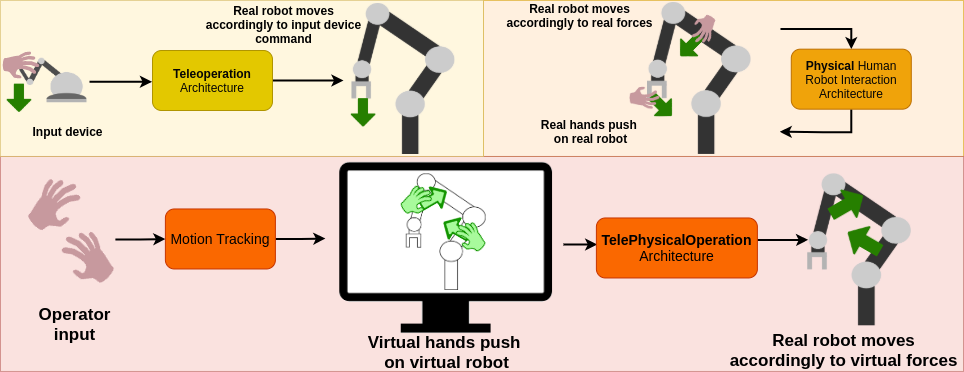
\includegraphics[width=0.85\linewidth]{img/TPOScheme}
	\caption{Concept of TelePhysicalOperation. Above, schematics of the traditional teleoperation and the physical human robot interaction interfaces. Below, the scheme of TelePhysicalOperation, derived by the combination of the two above controlling interfaces}
	\label{fig:tposcheme}
\end{figure}

By selecting specific control points on the robot kinematic chains, the operator can apply virtual forces that in a remote manner resembles the real applied forces of a physical human robot interaction exploited to guide the robot during a teaching/collaborative task. Thus, the proposed method permits to command the robot keeping a safe distance but also exploring the intuitiveness of the physical interaction. 
%
%\begin{figure}[H]
%	\centering
%	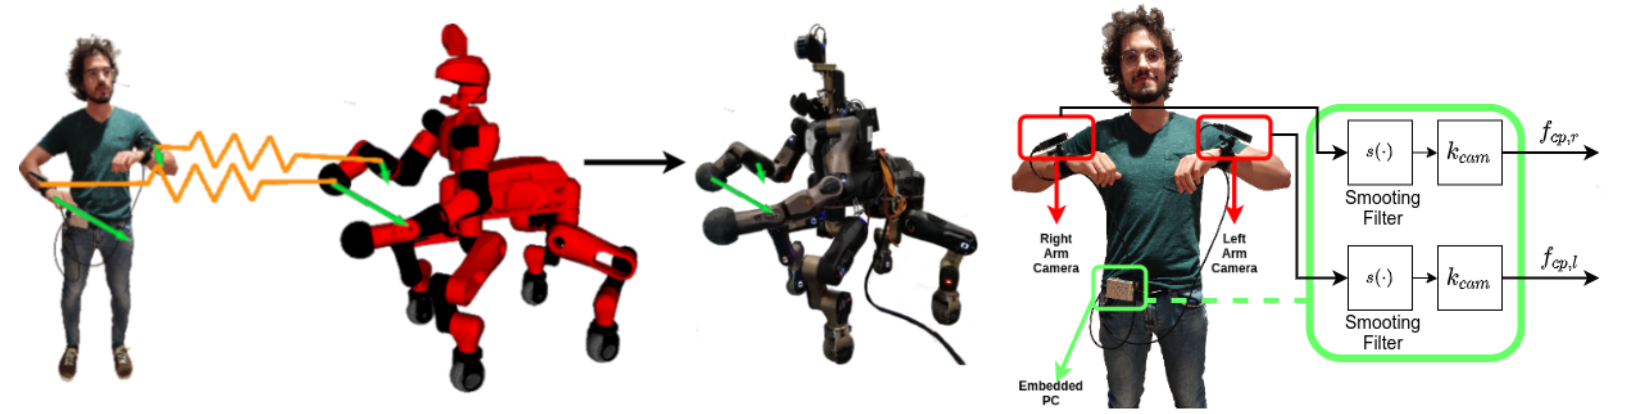
\includegraphics[width=0.9\linewidth]{img/TPOConcept}
%	\caption{On the right, the TelePhysicalOperation concept follows a \enquote{Marionette} type interaction: the operator generates virtual forces that can be selectively applied on specific locations on the robot segments. On the left, the TPO suit, the motion tracking interface used to gather operator arm movements and generate virtual forces $\boldsymbol{f}_{cp}$. }
%	\label{fig:tpoconcept}
%\end{figure}
%
The virtual forces are applied along the kinematic chain of the robot, which responds regulating its motion to comply with them as in a compliant physical human-robot interaction. The virtual forces are generated by virtual springs which link the arms of the human operator and the selected robot body parts, resembling a \enquote{Marionette} motion generation interface. The interface allows to virtually interact with the robot arms, hence controlling the robot manipulation ability, or with the body, hence controlling the robot mobility ability.
%
The virtual forces are generated through the motion of the operator arms. To track such motions, we make use of a lightweight and low-cost motion capture solution based on Visual-Simultaneous and Localization Mapping (V-SLAM) tracking cameras, worn on the operator wrists. In such a way, the movements of the user arms are associated with the elongation of the virtual spring used to compute the final virtual force that will be applied to the selected robot body part.

We conducted a series of experiment with the CENTAURO~\cite{Centauro2} robot [J.1]. For example, in \figurename~\ref{fig:tpoexp}, with the application of two virtual forces on two different points of the same arm of the robot, the operator can first activate the shoulder and the elbow joints to go over the obstacles (first image) and then bend the wrist to reach the button to be pressed from above (second and third images).   

\begin{figure}[H]
	\centering
	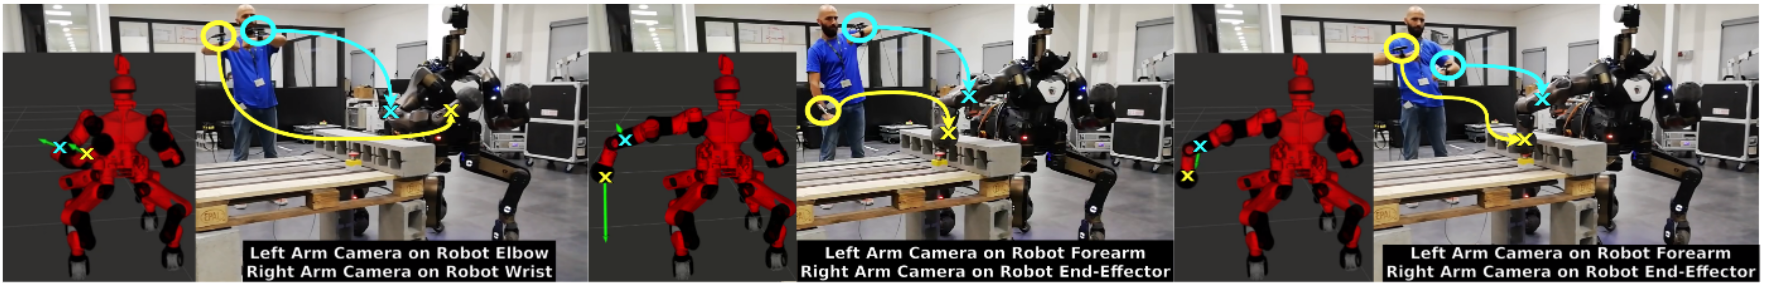
\includegraphics[width=0.95\linewidth]{img/tpoExp}
	\caption{In this experiment the goal is to press a button obstructed by some bricks. The cyan and yellow marks indicate where the virtual forces are applied by the operator. The robot visualization (RViz) shows the input directions commanded by the user (green arrows).}
	\label{fig:tpoexp}
\end{figure}


\subsection{Enhancing the Teleoperation Interfaces}
One common challenge with mobile manipulators is that both the robot arm(s) and the mobile platform must be considered when performing a locomanipulation tasks. Indeed, a change of control mode (from arm to mobile base and vice versa) is necessary each time the operator wants to move the mobile base or the arm, an operation that is repetitive and may increase the operator effort and the task execution time. As an alternative more input interfaces to control at the same time the base and the arm may be exploited, but this may augment the operator burden. To face this challenge, it is necessary to provide the robot with more autonomy, for example with whole-body controllers or other kind of techniques to switch automatically the control mode.
To address this problem, we have proposed a shared control interface for locomanipulation tasks to automatically generate mobile base motions even when only the arm is commanded [C.3]. In such a way, the operator can control exclusively the arm, without taking care of changing the control modality from the arm to the mobile base, and without taking care of the limited workspace of the arm. The proposed interface, integrated in the TelePhysicalOperation architecture, considers the manipulability level of the arm~\cite{Yoshi1985}, a measure strictly related to the kinematic singularities of the limb. If the robotic arm reaches a workspace region in which the manipulability in the direction of the applied virtual force is low, the generated motion is gradually switched to the mobile base. This permits to reach the desired end-effector goal without the necessity of switching from arm control to mobile base control, and assuring that the manipulability does not decrease beyond a defined threshold. 

In some scenarios, other autonomy features are necessary to accomplish successfully a task. In [C.3], [C.4] the mentioned manipulability-aware shared locomanipulation teleoperation has been enhanced with a strategy to regulate automatically the grasping forces on a object bi-manually transported by the robot \figurename~\ref{fig:tpoexpbox}.
In this way, the user is required to only command the object velocities (generating virtual forces from his/her arm movements), without worrying about arms manipulability, about switching from arms control to locomotion control, and about the grasping forces necessary to transport the load without dropping or damaging it.

\begin{figure}[H]
	\centering
	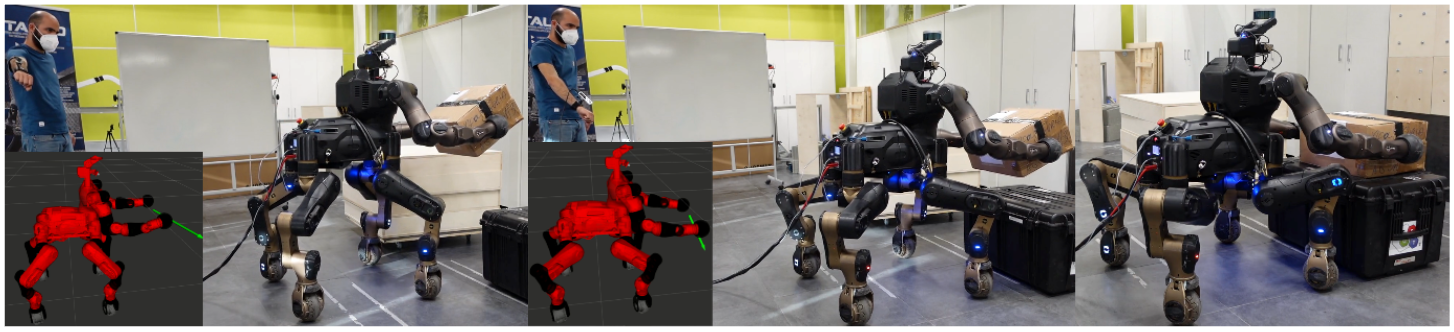
\includegraphics[width=0.9\linewidth]{img/tpoexpbox}
	\caption{The robot is teleoperated to transport the load to a location. The manipulability-aware shared locomotion is combined with a bimanual grasping feature to autonomously regulate the grasping forces applied on the object while accepting the operator commanded object velocities (shown as the green arrows in the robot visualization).}
	\label{fig:tpoexpbox}
\end{figure}

In parallel, haptic feedback have been explored [C.8]. Indeed, certain types of information about the status of the robot or of the task can not been transmitted to the user through a monitor or by watching directly the robot. To address the challenge, and further improve the TelePhysicalOperation paradigm, we have developed a sensorimotor interface~\cite{prattichizzo2021human} and integrated it into the TPO suit. In particular, the user wears two rings and two armbands, which can deliver vibration and skin indentation stimuli. 
The rings are also endowed with two small push buttons, providing additional input possibilities that, in the previous TPO works, had required the presence of an additional operator. Skin indentation stimuli are sent to the user to increase his/her awareness of the control command delivered to the robot and of the robot-environment interaction, whereas vibrations are used as acknowledgments about the execution of the command associated with a button.
User study evaluation with naive users teleoperating the CENTAURO robot showed a positive outcome for the devices integrated in the interface, assessing only a slight increase in the complexity of the additional devices worn.


\subsection{Laser-based Visual Teleoperation}
In the direction of simplify the control of complex robots, another intuitive teleoperation interface has been explored, developing a visual servoing framework which permits to control a robot with a laser emitter [J.4, C.6, C.7]. By pointing the laser in the environment, the operator is able to command even highly articulated robots effortlessly and efficiently. 
The perception layer that tracks the laser spot implements a neural network solution, based on YOLO~\cite{yolov5}. This has resulted to be a much faster and robust solution compared to common computer vision techniques, permitting to promptly detect goal position changes. 

In the main work that exploit this interface [J.4], the robot behavior is built around a Behaviour Tree, a flexible and modular planning structure, easily adaptable to different robot and different tasks. The evaluation of such architecture has been validated on the CENTAURO robot in a series of tasks, for example in a pick-and-place mission combining the manipulation and the locomotion ability of the robot (\figurename~\ref{fig:pickAndPlacePhoto}).

\begin{figure}[H]
	\centering
	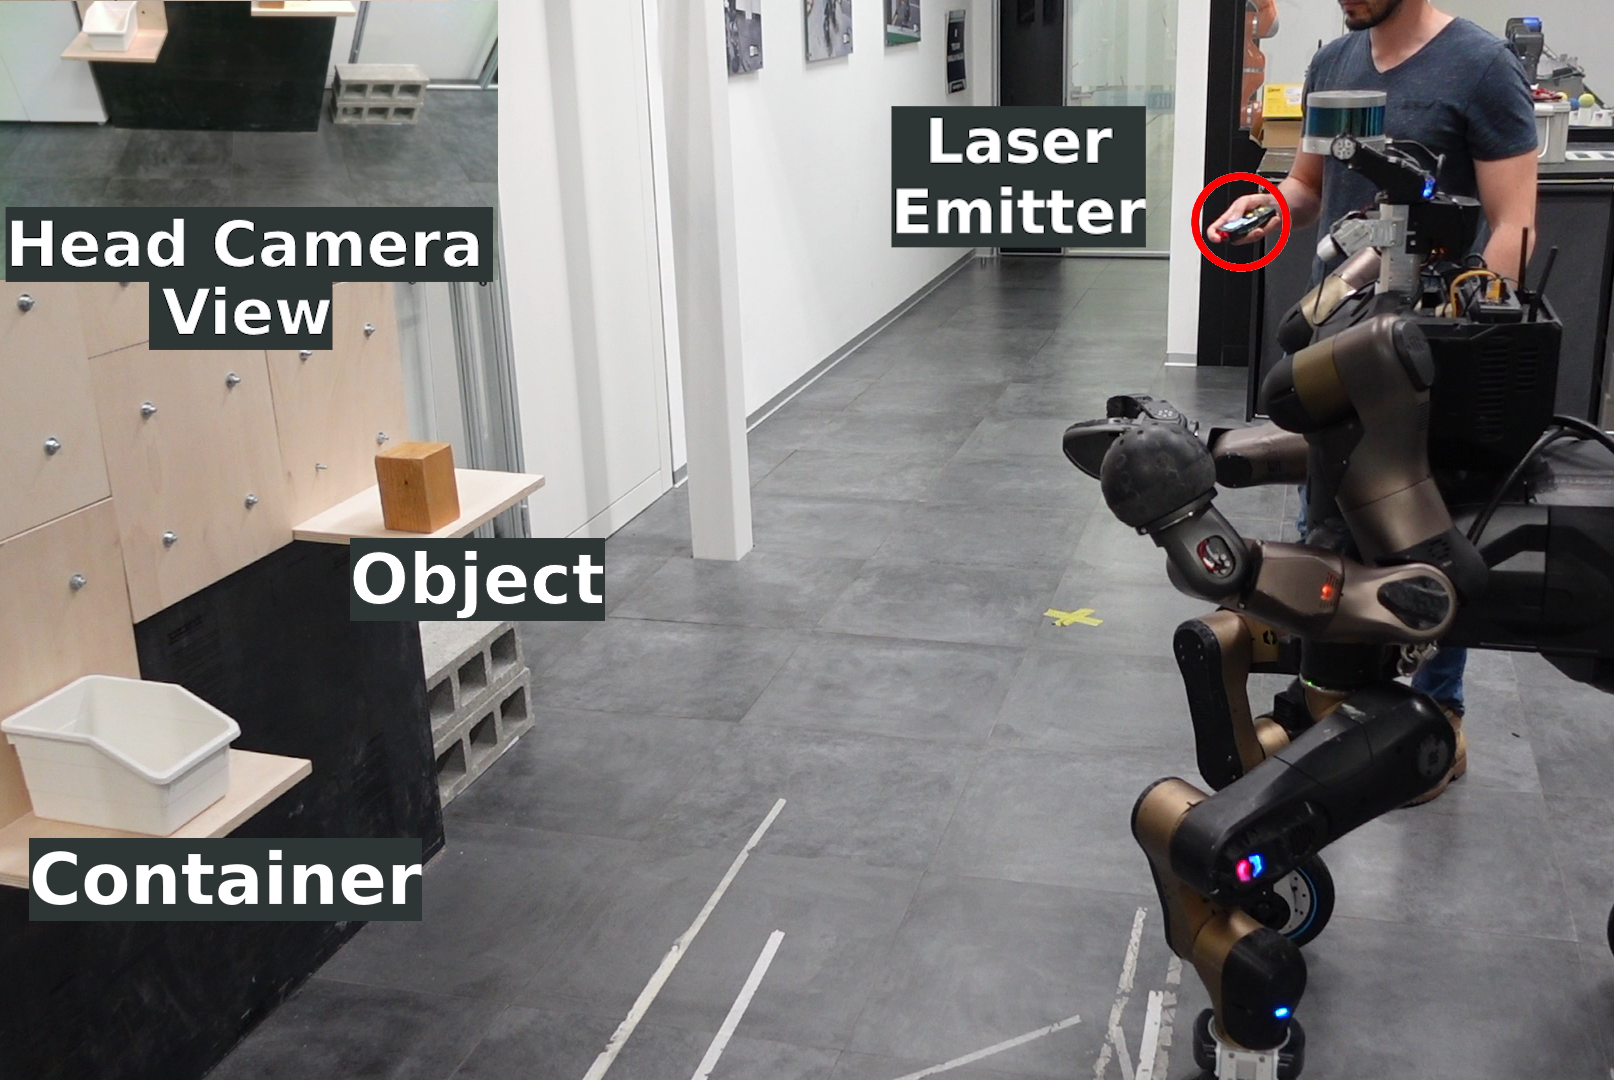
\includegraphics[height=0.2\linewidth, keepaspectratio]{img/grasp1Edited}
	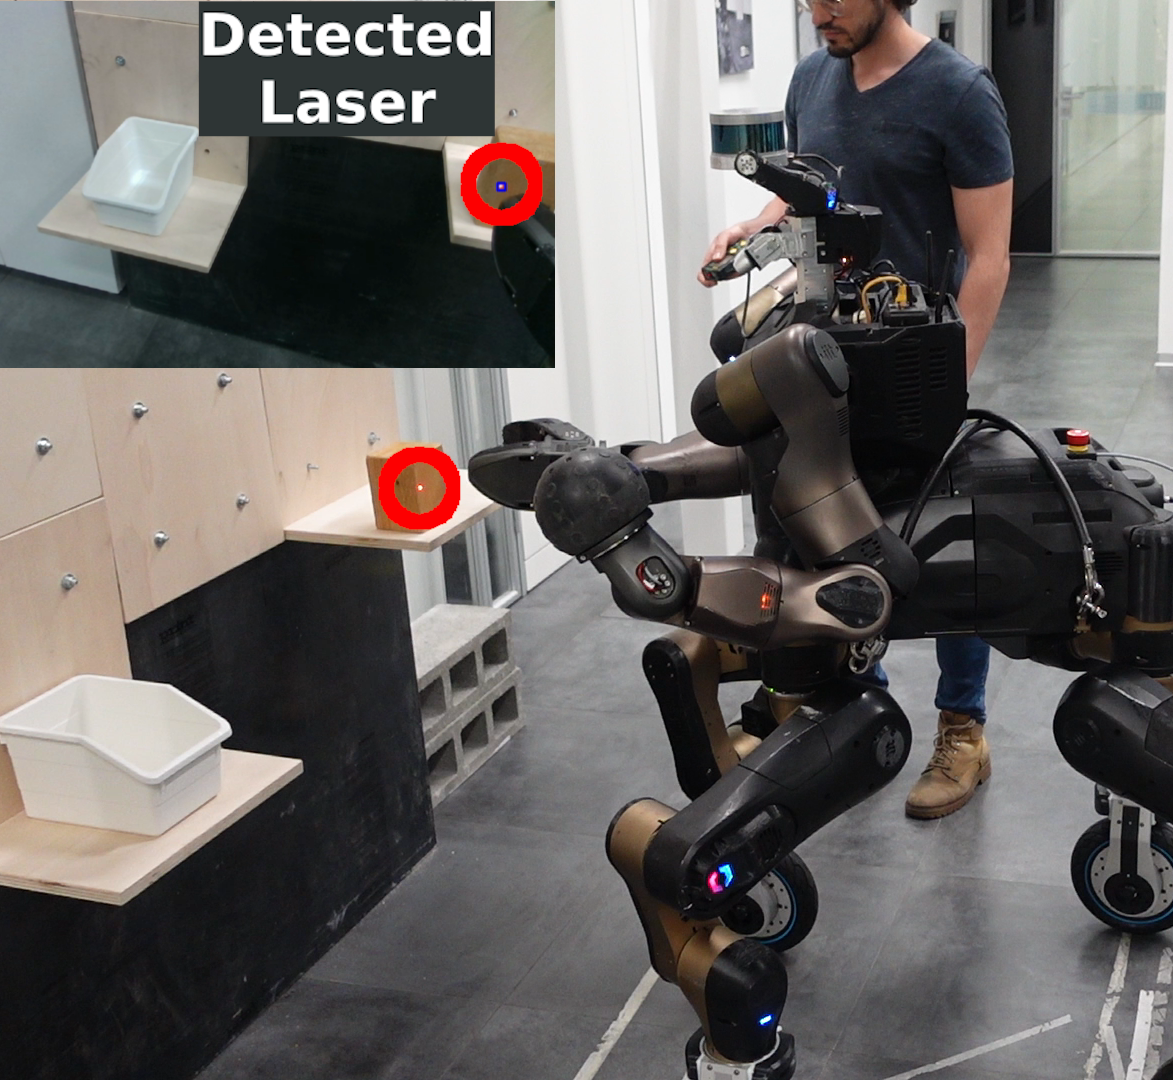
\includegraphics[height=0.2\linewidth, keepaspectratio]{img/grasp2Edited}	
	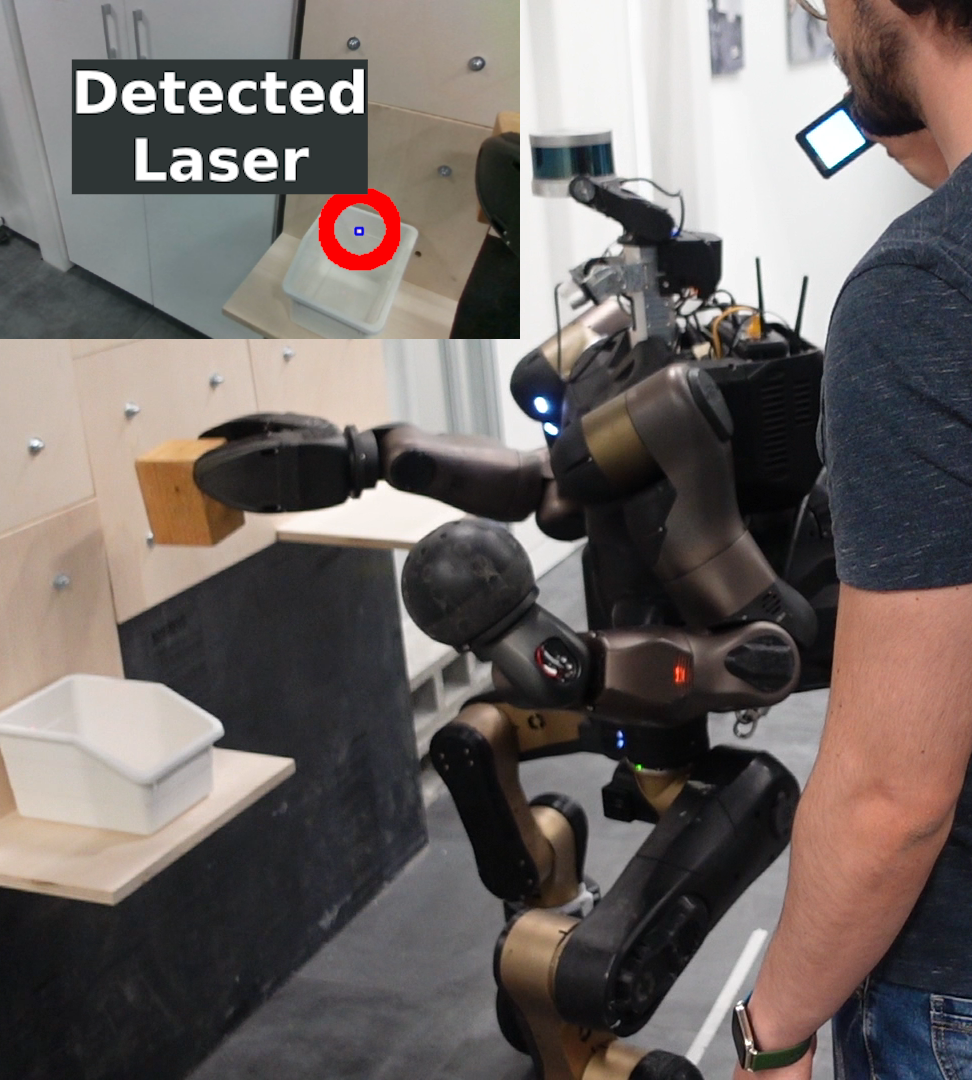
\includegraphics[height=0.2\linewidth, keepaspectratio]{img/grasp4Edited}
	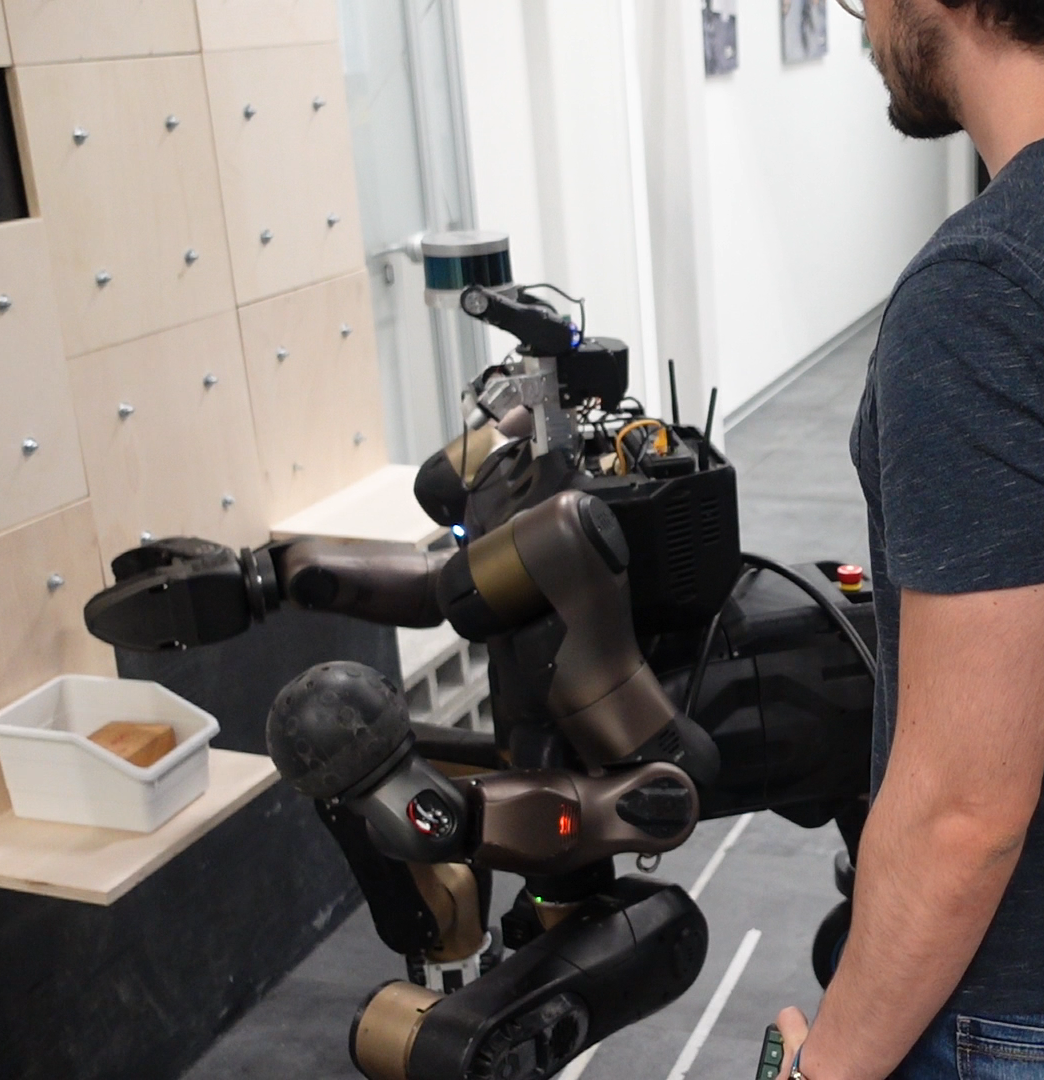
\includegraphics[height=0.2\linewidth, keepaspectratio]{img/grasp5Edited}
	\caption{Sequences of the pick-and-place experiment. The operator guides the robot toward the object, to place it into the container. Once the end-effector is in position, the user requests to grasp/release the object, interrupting temporarily the tracking of the laser.}
	\label{fig:pickAndPlacePhoto}	
\end{figure}

In other works [C.6 C.7], the laser-based teleoperation interface has been exploited for an assistive scenario. The target are impaired arm users, which have limited abilities on one or both arms, and need help for Activities of Daily Living (ADL). Hence, the laser is worn on the user's head permitting to command a fixed manipulator with head movements. Two control modalities are available, activated based on where the laser is pointed. 
When the laser is pointed onto the environment, the framework generates and executes a collision free trajectory toward the indicated goal. 
Instead, with the second modality, the user can \enquote{click} the keys of a paper keyboard by projecting the laser onto them. The keyboard permits to control the robot end-effector by commanding Cartesian velocities with a direction represented by the selected key. 

In \figurename~\ref{fig:pane3-frames}, it is reported an ADL task executed with the interface proposed, where the user, simulating an impairment on his right arm, commands the robot to hold the bread that must be cut.
In the leftmost image, it is shown how the user exploits the first modality to command the arm above the bread. In the second image, the user finalizes the robot end-effector position and close the gripper by projecting the laser on the keyboard.

\begin{figure}[H]
	\centering
 	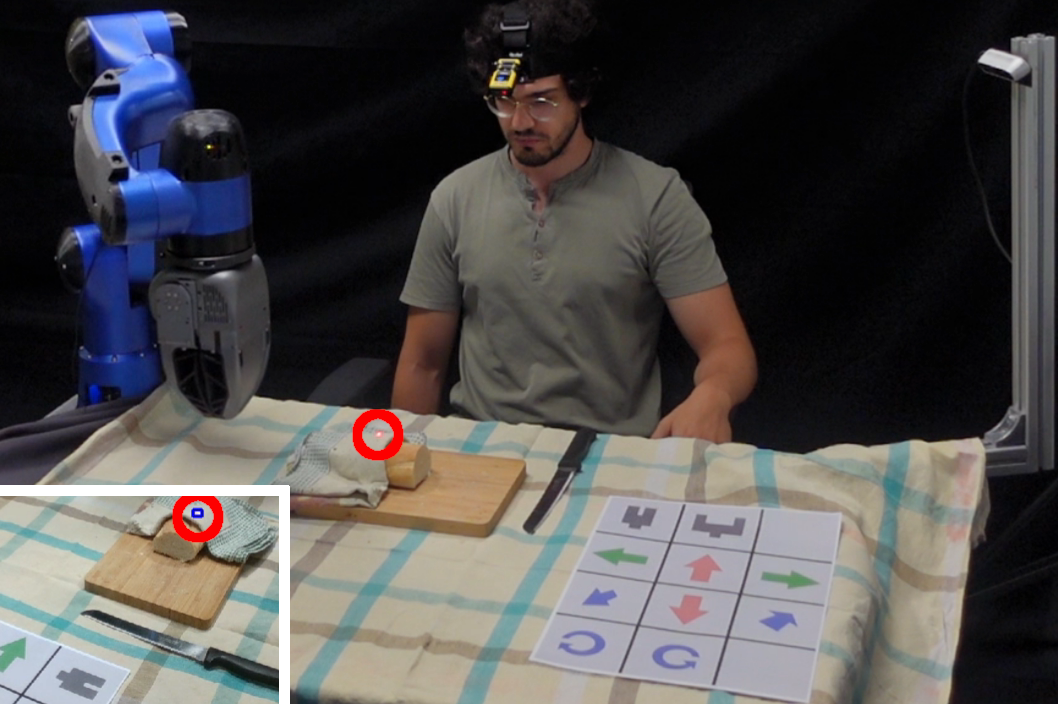
\includegraphics[width=0.22\linewidth]{img/pane-frame0edited.png}
	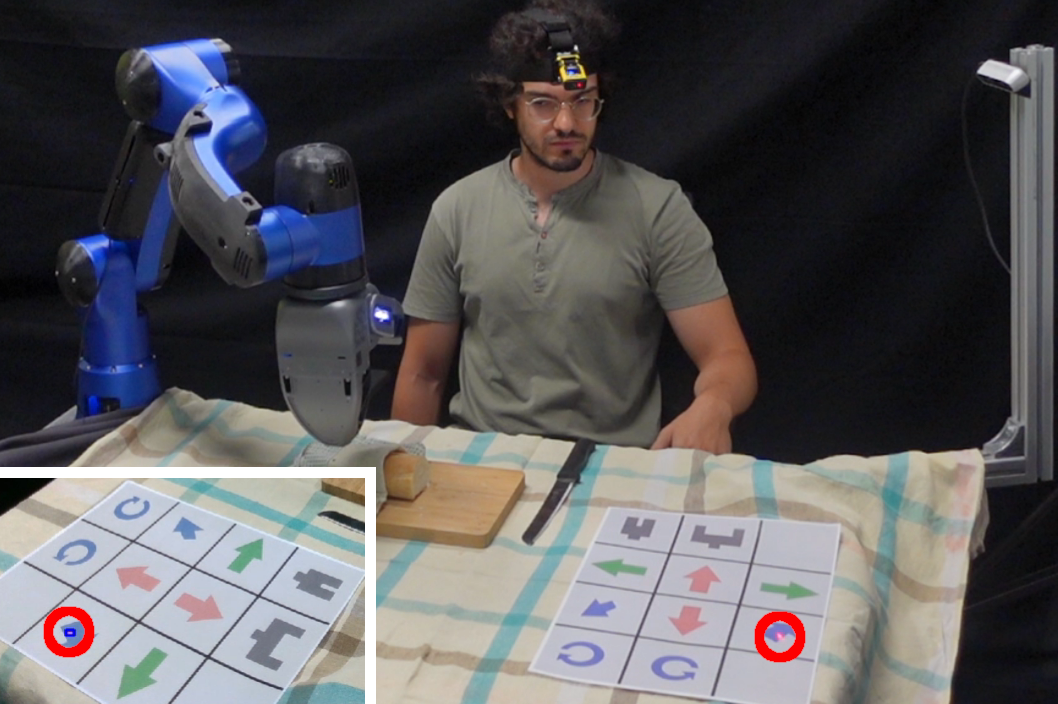
\includegraphics[width=0.22\linewidth]{img/pane-frame1edited.png}
	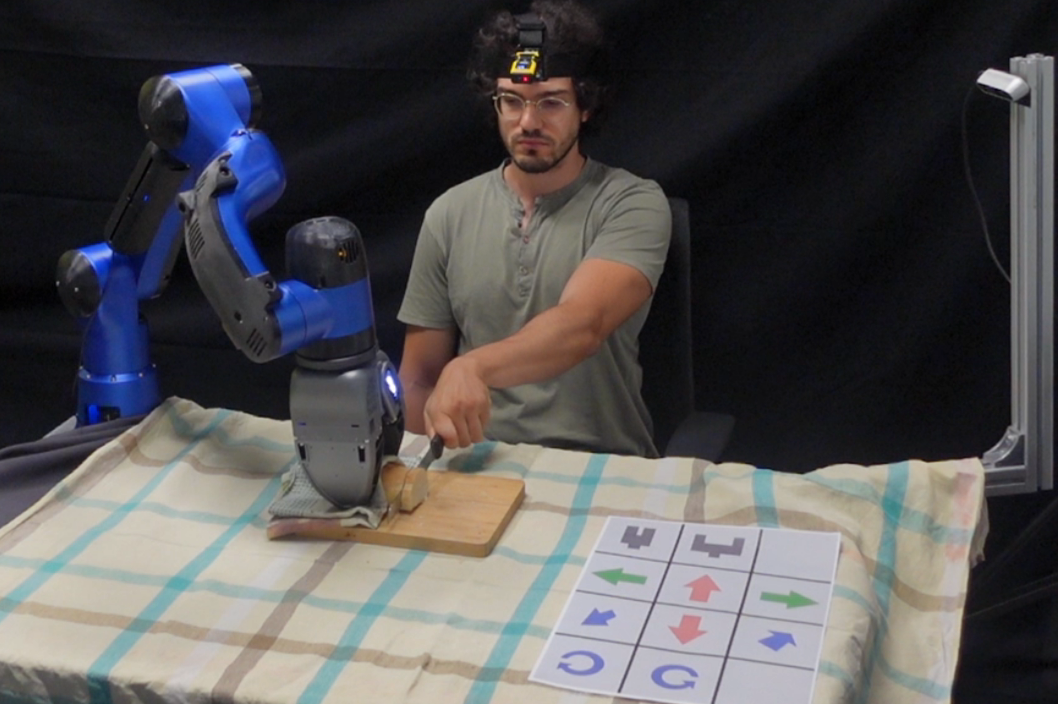
\includegraphics[width=0.22\linewidth]{img/pane-frame2edited.png}
	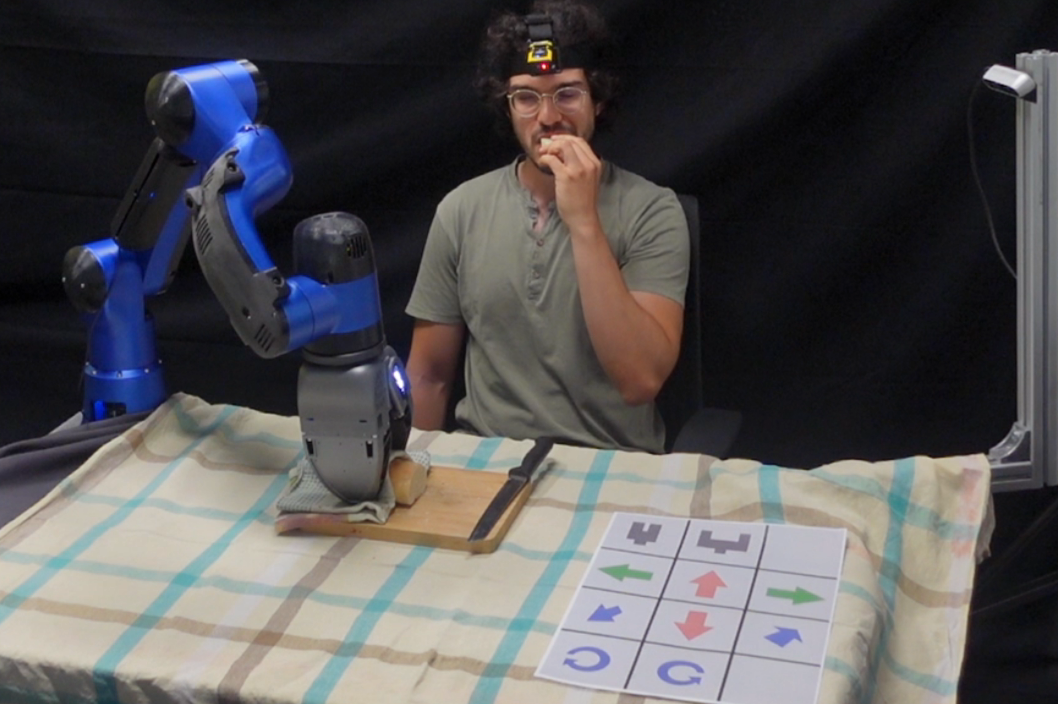
\includegraphics[width=0.22\linewidth]{img/pane-frame3edited.png}
	\caption{Sequences of the \enquote{cutting bread} experiment, with the camera view added in the frames when the robot is commanded, showing the detected laser spot.}
	\label{fig:pane3-frames}
\end{figure}


\newpage
\section{Training}
%List the courses, schools, training activities followed during this academic year.
I attended the following courses, offered by University of Genova:
\begin{table}[H]
	\begin{center}
		\renewcommand{\arraystretch}{1.3} % Adjust the vertical spacing
		\setlength{\tabcolsep}{8pt} % Adjust the horizontal spacing
		\begin{tabular}{P{10cm} P{3cm} P{0.8cm} P{0.8cm}}
			\toprule
			\textbf{Activity name} & \textbf{Professor} & \textbf{CFU} & \textbf{Year} \\ 
			\midrule
			Interaction in Virtual and Augmented reality & M. Chessa & none & 1$^{st}$ \\
			\midrule
			An Introduction to Open Science and Research Data Management & V. Pasquale - A.M. Pastorini & 3 & 1$^{st}$ \\ 
			\midrule
			Ethics and Bioethics in Bioengineering and Robotics & L. Battistuzzi & 5 & 1$^{st}$ \\
			\midrule
			Modern C++ & M. Accame & 5 & 1$^{st}$ \\
			\midrule
			Model Predictive Control and Applications & M. Gaggero & none & 1$^{st}$ \\
			\midrule
			An introduction to spatial (6D) vectors and their use in robot dynamics & R. Featherstone & none & 1$^{st}$ \\ 
			\midrule
			Computational Robot Dynamics & R. Featherstone & 5 & 1$^{st}$ \\ 
			\midrule
			Introduction to physical Human-Robot Interaction & J. Zenzeri & 5 & $1^{st}$ \\	
			\midrule
			Theatrical techniques for public speaking & A. Sgorbissa & 5 & $1^{st}$ \\ 
			\bottomrule
			Grant Writing & C. Leone & 5 & 1$^{st}$ \\ 
			\midrule
			Paper Writing & M. Marchese & 5 & $1^{st}$ \\ 
			\midrule 
			Introduction to space exploration & F. Malerba & 5 & 2$^{nd}$ \\
			\midrule
			Mechatronics and AI & G. Marchello & none & 2$^{nd}$\\
			\bottomrule
		\end{tabular}
	\end{center}
	\caption{Training Activities}
\end{table}

I attended the following summer schools:
\begin{table}[H]
	\begin{center}
		\renewcommand{\arraystretch}{1.3} % Adjust the vertical spacing
		\setlength{\tabcolsep}{8pt} % Adjust the horizontal spacing
		\begin{tabular}{P{10cm} P{3cm} P{0.8cm} P{0.8cm}}
			\toprule
			\textbf{Activity name} & \textbf{Organizer} & \textbf{CFU} & \textbf{Year} \\ 
			\midrule
			EECI 2023 International Graduate School on Control & ETH, Zurich & 3 & 3$^{rd}$ \\ 
			\midrule
			Summer School on Autonomous Mobile Robotics in the framework of Industry 4.0  & Unisalento, Lecce & 5 & 2$^{nd}$ \\ 
			\midrule
			IEEE RAS Summer School on multi-robot systems & CTU, Prague & 3 & 2$^{nd}$ \\	
			\bottomrule
		\end{tabular}
	\end{center}
	\caption{Summer Schools}
\end{table}

\section{Publication record}
\subsection{Peer reviewed journal papers}
\begin{enumerate}[label={[J.\arabic*]}]
	\item \fullcite{TPO}
	\item \fullcite{ROSEE}	
	\item \fullcite{Muratore2023}
	\item \fullcite{LaserJournal}
\end{enumerate}
\subsection{Peer-reviewed conference proceedings}
\begin{enumerate}[label={[C.\arabic*]}]
	\item \fullcite{RoseePaper}
	\item \fullcite{RoseePaperLiana}
	\item \fullcite{TPO2}
	\item \fullcite{TPOIRIM}
	\item \fullcite{TPO3}
	\item \fullcite{LaserHumanoids}
	\item \fullcite{Bertoni2023}
	\item \fullcite{TPO4}
\end{enumerate}
\section{Other activities}
\subsection{\textbf{I Year}}
\begin{itemize}
	\item Presentation of the \enquote{ROS End-Effector} project at the \textit{ROSIN FTP Webinar Series, session 5}
	(19.11.2020) \url{https://www.youtube.com/watch?v=rVzLnDJEs-I}
\end{itemize}

\subsection{\textbf{II Year}}
\begin{itemize}
	\item Presentation of the paper titled \enquote{Towards an Open-Source Hardware Agnostic Framework for Robotic End-Effectors Control} [C.1] at the \textit{International Conference on Advanced Robotics ICAR} (December 07-10, 2022, Ljubljana, Slovenia (virtual event)) \url{https://icar-2021.org/}
	
	\item Presentation of the paper titled \enquote{TelePhysicalOperation: Remote Robot Control Based on a Virtual “Marionette” Type Interaction Interface} [J.1] at the \textit{IEEE International Conference on Robotics and Automation ICRA} (May 23-27, 2022, Philadelphia (PA), USA)
	\url{https://www.icra2022.org/}
	
	\item Co-presentation of the \enquote{Exploiting ROS 2 to facilitate end-effectors integration and control} talk at the \textit{ROSCON22 conference} (October 19-21, 2022, Kyoto, Japan) \url{https://roscon.ros.org/2022/}
	
	\item Presentation of the paper titled \enquote{Manipulability-aware shared locomanipulation motion generation for teleoperation of mobile manipulators} [C.3] at the \textit{IEEE/RSJ International Conference on Intelligent Robots and Systems} (October 23-27, 2022, Kyoto, Japan)
	\url{https://iros2022.org/}
\end{itemize}

\subsection{\textbf{III Year}}
\begin{itemize}
	\item Presentation of the paper titled \enquote{A shared telemanipulation interface to facilitate
	bimanual grasping and transportation of objects of unknown mass} [C.5] at the \textit{IEEE-RAS International Conference on Humanoid Robots} (November 28–30, 2022, Ginowan, Okinawa, Japan) \url{https://www.humanoids2022.org/}	
		
	\item Co-presentation of the \enquote{ROS End-Effector: A hardware-agnostic framework to facilitate end-effectors integration, planning and control with the ROS2 middleware} talk at the \textit{ROS-Industrial Conference} (December 15–16, 2022, Stuttgart, Germany (virtual partecipation)) \url{https://rosindustrial.org/rosindustrial-conference-2022}
	
	\item Participation at the \textit{ROSCON23 conference} (October 18-20, 2023, New Orleans, USA) \url{https://roscon.ros.org/2023/}
	
\end{itemize}

\cleardoublepage

%\bibliographystyle{unsrt}
%\bibliography{refs/refs.bib}
\printbibliography[notcategory=dontbib]

\end{document}
